\documentclass[journal,12pt,twocolumn]{IEEEtran}

\usepackage{setspace}
\usepackage{gensymb}
\singlespacing
\usepackage[cmex10]{amsmath}

\usepackage{amsthm}
\usepackage{amsmath,amssymb}
\usepackage{mathrsfs}
\usepackage{txfonts}
\usepackage{stfloats}
\usepackage{bm}
\usepackage{cite}
\usepackage{cases}
\usepackage{subfig}

\usepackage{longtable}
\usepackage{multirow}
\usepackage{float}
\usepackage{enumitem}
\usepackage{mathtools}
\usepackage{steinmetz}
\usepackage{tikz}
\usepackage{circuitikz}
\usepackage{verbatim}
\usepackage{tfrupee}
\usepackage[breaklinks=true]{hyperref}
\usepackage{graphicx}
\usepackage{tkz-euclide}
\usepackage{stackengine}
\usetikzlibrary{calc,math}
\usepackage{listings}
    \usepackage{color}                                            %%
    \usepackage{array}                                            %%
    \usepackage{longtable}                                        %%
    \usepackage{calc}                                             %%
    \usepackage{multirow}                                         %%
    \usepackage{hhline}                                           %%
    \usepackage{ifthen}                                           %%
    \usepackage{lscape}     
\usepackage{multicol}
\usepackage{chngcntr}
\usepackage{bm}
\DeclareMathOperator*{\Res}{Res}

\renewcommand\thesection{\arabic{section}}
\renewcommand\thesubsection{\thesection.\arabic{subsection}}
\renewcommand\thesubsubsection{\thesubsection.\arabic{subsubsection}}

\renewcommand\thesectiondis{\arabic{section}}
\renewcommand\thesubsectiondis{\thesectiondis.\arabic{subsection}}
\renewcommand\thesubsubsectiondis{\thesubsectiondis.\arabic{subsubsection}}


\hyphenation{op-tical net-works semi-conduc-tor}
\def\inputGnumericTable{}                                 %%

\lstset{
%language=C,
frame=single, 
breaklines=true,
columns=fullflexible
}
\makeatletter
\setlength{\@fptop}{0pt}
\makeatother
\begin{document}

\newcommand{\BEQA}{\begin{eqnarray}}
\newcommand{\EEQA}{\end{eqnarray}}
\newcommand{\define}{\stackrel{\triangle}{=}}
\bibliographystyle{IEEEtran}
\raggedbottom
\setlength{\parindent}{0pt}
\providecommand{\mbf}{\mathbf}
\providecommand{\pr}[1]{\ensuremath{\Pr\left(#1\right)}}
\providecommand{\qfunc}[1]{\ensuremath{Q\left(#1\right)}}
\providecommand{\sbrak}[1]{\ensuremath{{}\left[#1\right]}}
\providecommand{\lsbrak}[1]{\ensuremath{{}\left[#1\right.}}
\providecommand{\rsbrak}[1]{\ensuremath{{}\left.#1\right]}}
\providecommand{\brak}[1]{\ensuremath{\left(#1\right)}}
\providecommand{\lbrak}[1]{\ensuremath{\left(#1\right.}}
\providecommand{\rbrak}[1]{\ensuremath{\left.#1\right)}}
\providecommand{\cbrak}[1]{\ensuremath{\left\{#1\right\}}}
\providecommand{\lcbrak}[1]{\ensuremath{\left\{#1\right.}}
\providecommand{\rcbrak}[1]{\ensuremath{\left.#1\right\}}}
\DeclarePairedDelimiter\ceil{\lceil}{\rceil}
\DeclarePairedDelimiter\floor{\lfloor}{\rfloor}
\theoremstyle{remark}
\newtheorem{rem}{Remark}
\newcommand{\sgn}{\mathop{\mathrm{sgn}}}
\providecommand{\abs}[1]{\vert#1\vert}
\providecommand{\res}[1]{\Res\displaylimits_{#1}} 
\providecommand{\norm}[1]{\lVert#1\rVert}
%\providecommand{\norm}[1]{\lVert#1\rVert}
\providecommand{\mtx}[1]{\mathbf{#1}}
\providecommand{\mean}[1]{E[ #1 ]}
\providecommand{\fourier}{\overset{\mathcal{F}}{ \rightleftharpoons}}
%\providecommand{\hilbert}{\overset{\mathcal{H}}{ \rightleftharpoons}}
\providecommand{\system}{\overset{\mathcal{H}}{ \longleftrightarrow}}
	%\newcommand{\solution}[2]{\textbf{Solution:}{#1}}
\newcommand{\solution}{\noindent \textbf{Solution: }}
\newcommand{\cosec}{\,\text{cosec}\,}
\newcommand*{\permcomb}[4][0mu]{{{}^{#3}\mkern#1#2_{#4}}}
\newcommand*{\perm}[1][-3mu]{\permcomb[#1]{P}}
\newcommand*{\comb}[1][-1mu]{\permcomb[#1]{C}}
\newcommand\xrowht[2][0]{\addstackgap[.5\dimexpr#2\relax]{\vphantom{#1}}}
\providecommand{\dec}[2]{\ensuremath{\overset{#1}{\underset{#2}{\gtrless}}}}
\newcommand{\myvec}[1]{\ensuremath{\begin{pmatrix}#1\end{pmatrix}}}
\newcommand{\mydet}[1]{\ensuremath{\begin{vmatrix}#1\end{vmatrix}}}
\numberwithin{equation}{subsection}
\makeatletter
\@addtoreset{figure}{problem}
\makeatother
\let\StandardTheFigure\thefigure
\let\vec\mathbf
\renewcommand{\thefigure}{\theproblem}
\def\putbox#1#2#3{\makebox[0in][l]{\makebox[#1][l]{}\raisebox{\baselineskip}[0in][0in]{\raisebox{#2}[0in][0in]{#3}}}}
     \def\rightbox#1{\makebox[0in][r]{#1}}
     \def\centbox#1{\makebox[0in]{#1}}
     \def\topbox#1{\raisebox{-\baselineskip}[0in][0in]{#1}}
     \def\midbox#1{\raisebox{-0.5\baselineskip}[0in][0in]{#1}}
\vspace{3cm}
\title{Assignment 9}
\author{Chirag Mehta - AI20BTECH11006}
\maketitle
\newpage
\bigskip
\renewcommand{\thefigure}{\theenumi}
\renewcommand{\thetable}{\theenumi}
Download all python codes from 
\begin{lstlisting}
https://github.com/cmapsi/AI1103-Probability-and-random-variables/tree/main/Assignment-9/codes
\end{lstlisting}
and latex-tikz codes from 
\begin{lstlisting}
https://github.com/cmapsi/AI1103-Probability-and-random-variables/blob/main/Assignment-9/main.tex
\end{lstlisting}
\section{Problem}
(CSIR UGC NET EXAM (Dec 2015), Q.109)\\
Suppose
$\begin{pmatrix}
X\\
Y
\end{pmatrix}$ is a random vector such that the marginal distribution of $X$ and the marginal distribution of $Y$ are the same and each is normally distributed with mean 0 and variance 1. Then, which of the following conditions imply independence of $X$ and $Y?$
\begin{enumerate}
\item Cov$\brak{X,Y}=0$
\item $aX+bY$ is normally distributed with mean 0 and variance $a^2+b^2$ for all real $a$ and $b$
\item $\pr{X\le 0, Y\le0}=\frac{1}{4}$
\item $E\sbrak{e^{itX+isY}}=E\sbrak{e^{itX}}E\sbrak{e^{isY}}$ for all real $s$ and $t$
\end{enumerate}
\section{solution}
An important property of dirac delta function that will be used at multiple ocassions in this solution is
\begin{align}
\displaystyle\int\limits_{-\infty}^{\infty} f(x)\delta(x-a)dx=f(a) \label{eq:dirac}
\end{align}
Given $X\sim N\brak{0,1}, Y\sim N(0,1)$
\begin{enumerate}
\item
\begin{align}
Cov(X,Y)=0\\
E\sbrak{XY}-E\sbrak{X}E\sbrak{Y}=0\\
E\sbrak{XY}=0\\
\displaystyle \int\limits_{-\infty}^{\infty} \int\limits_{-\infty}^{\infty}xyf_{XY}(x,y) dxdy=0
\end{align}
This doesn't imply independence. Counter example given below\\
Lets consider a case where $X$ and $Y$ are dependent based on the following relation, $Y$ being independent of $K$
\begin{align}
X=KY \label{eq:case}
\end{align}
PMF for $K$ is given as
\begin{align}
p_K(k)=
\begin{cases}
\frac{1}{2} &k=1\\
\frac{1}{2} & k=-1\\
0 & \text{otherwise}
\end{cases}
\end{align}
A simulation is given below, Y is gaussian, then X also follows gaussian
\begin{figure}[H]
\centering
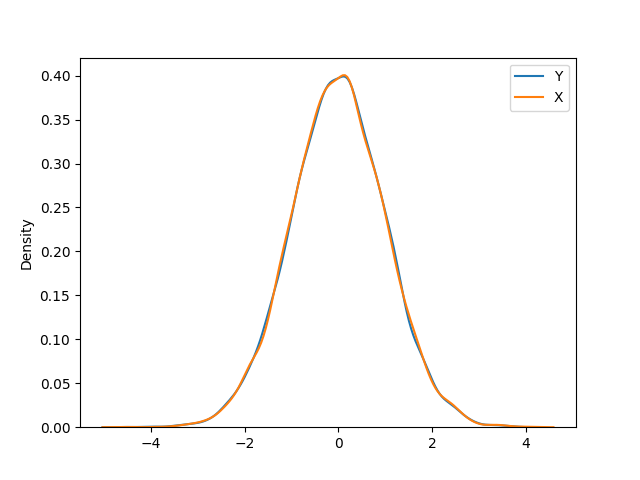
\includegraphics[width=\linewidth]{figure/fig}
\caption{X and Y, if Y is normal}
\label{plot}
\end{figure}
Theoretically it can be proved in the following manner,
Since $K$ and $Y$ are independent
\begin{align}
f_X(x)&=\pr{K=1}f_Y(x)+\pr{K=-1}f_Y(-x)\\
&=\frac{1}{2}\brak{f_Y(x)+f_Y(-x)}\\
&=f_Y(x)
\end{align}
Therefore, $X$ follows identical but not independent distribution as $Y$, An alternative proof is given below as a proof for marginal probability\\
Now consider that $X$ is normally distributed, we will establish $Y$ is also normally distributed.
The joint probability distribution is therefore
\begin{align}
f_{XY}(x,y)&=f_{X|Y}(x|y)f_X(x)\nonumber \\
&=f_X(x)\frac{1}{2}(\delta(x+y)+\delta(x-y))\label{eq:counter}
\end{align}
The marginal probability distribution function for $X$ is given as
\begin{align}
\int\limits_{-\infty}^{\infty}f_X(x)\frac{1}{2}(\delta(x+y)+\delta(x-y)) dy
\end{align}
Using \eqref{eq:dirac}, we get
\begin{align}
\int\limits_{-\infty}^{\infty}f_X(x)\frac{1}{2}(\delta(x+y)+\delta(x-y))dy=f_X(x)
\end{align}
We know that $X\sim N(0,1)$, $f_X(x)$ represents gaussian probability distribution function.\\
Futher, using symmetry of \eqref{eq:case}, we can establish that marginal distribution of $Y$ is gaussian. Here is a proof anyways
\begin{align}
f_Y(y)=\int\limits_{-\infty}^{\infty}f_X(x)\frac{1}{2}(\delta(x+y)+\delta(x-y)) dx
\end{align}
Using \eqref{eq:dirac}, we get
\begin{align}
f_Y(y)=\frac{1}{2}\brak{f_X(y)+f_X(-y)}=f_X(y)
\end{align}
Since $Y$ has identical probability distribution function, $Y\sim N(0,1)$\\
The covariance is given as
\begin{align}
&Cov(X,Y)=E[XY]-E[X]E[Y]=E[XY]\\
&E[XY]=\int\limits_{-\infty}^{\infty}\int\limits_{-\infty}^{\infty}xyf_{XY}(x,y) dy dx
\end{align}
\begin{align}
=\int\limits_{-\infty}^{\infty}\int\limits_{-\infty}^{\infty}xyf_X(x)\frac{1}{2}(\delta(x+y)+\delta(x-y)) dy dx\\
=\int\limits_{-\infty}^{\infty} xf_X(x)\int\limits_{-\infty}^{\infty}y\frac{1}{2}(\delta(x+y)+\delta(x-y)) dy dx
\end{align}
Using \eqref{eq:dirac}
\begin{align}
E[XY]=\int\limits_{-\infty}^{\infty}xf_X(x)\frac{1}{2}(x-x)dx=0
\end{align}
\item
Defining the following matrices/vectors
\begin{table}[htp]
\centering
    \resizebox{0.7\columnwidth}{25mm}{
\begin{tabular}{ |c|c|c|} 
\hline
\textbf{vector/matrix} & \textbf{expression} \\
\hline\xrowht[()]{15pt}
$\boldsymbol{Z}$& $\begin{pmatrix} X &Y\end{pmatrix}^\top$\\
\hline\xrowht[()]{15pt}
$\boldsymbol{C}$&$\begin{pmatrix} a &b\end{pmatrix}^\top$  \\
\hline\xrowht[()]{15pt}
$\boldsymbol{\mu}$&$\begin{pmatrix} 0 &0\end{pmatrix}^\top$  \\
\hline\xrowht[()]{25pt}
$\boldsymbol{\Sigma}$&$\begin{pmatrix}1&\rho\\\rho&1\end{pmatrix}$ \xrowht[()]{20pt}\\
\hline
\end{tabular}}
\caption{vectors/matrices and their expressions}
\label{table1}
\end{table}
Given
\begin{align}
\boldsymbol{C^\top Z}\sim N\brak{0,a^2+b^2}
\end{align}
Since this is true for all $a$ and $b$, it is equivalent to $X$ and $Y$ being jointly gaussian
\begin{align}
\boldsymbol{Z}\sim N(\boldsymbol{\mu},\boldsymbol{\Sigma})
\end{align}
For correlated random variables $X$ and $Y$ in bivariate normal distribution, we have
\begin{align}
\sigma_{Z}^2=\displaystyle\sum_{i,j}\Sigma_{ij}\\
a^2+b^2=a^2+b^2+2\rho ab\\
\therefore \rho=0\label{eq:rho}
\end{align}
The joint distribution is given as
\begin{align}
f_{\boldsymbol{Z}}(x,y)=\frac{\text{exp}\brak{-\frac{1}{2}\brak{\boldsymbol{z-\mu}}^\top\boldsymbol{\Sigma}^{-1}\brak{\boldsymbol{z-\mu}}}}{\sqrt{(2\pi)^2\abs{\boldsymbol{\Sigma}}}}\\
f_{\boldsymbol{Z}}(x,y)=\frac{\text{exp}\brak{-\frac{1}{2}{\begin{pmatrix} x &y\end{pmatrix}} I_2{\begin{pmatrix} x &y\end{pmatrix}}^\top}}{\sqrt{(2\pi)^2}}
\end{align}
Where $I_2$ is the identity matrix of order 2
\begin{align}
f_{\boldsymbol{Z}}(x,y)=\frac{\text{exp}\brak{-\frac{1}{2}{\begin{pmatrix} x &y\end{pmatrix}} {\begin{pmatrix} x &y\end{pmatrix}}^\top}}{\sqrt{(2\pi)^2}}\\
f_{\boldsymbol{Z}}(x,y)=\frac{\text{exp}\brak{-\frac{1}{2}\brak{x^2+y^2}}}{\sqrt{(2\pi)^2}}=f_X(x)f_Y(y)
\end{align}
$\therefore$ \textbf{Option(2) is correct}, A simulation for bivariate gaussian is given below
\begin{figure}[H]
\centering
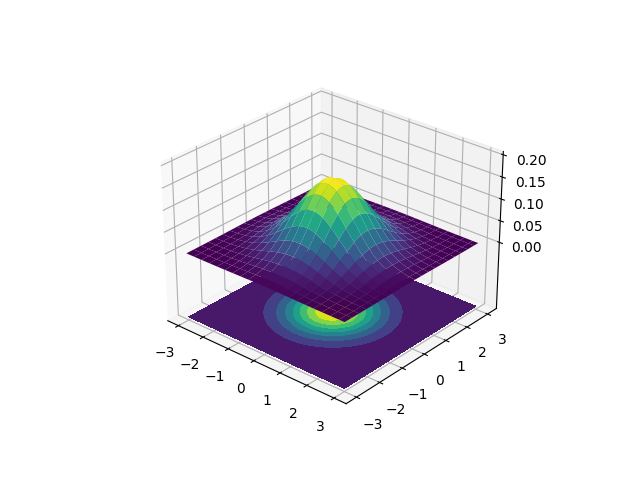
\includegraphics[width=\linewidth]{figure/plot}
\caption{bivariate gaussian while 0 mean vector and identity covariance matrix}
\label{plot}
\end{figure}
\item
\begin{align}
\pr{X\le 0, Y\le0}=\frac{1}{4}
\end{align}
This doesn't imply independence, it can be true even for dependent $X$ and $Y$, the counter example is \eqref{eq:counter}, the joint probability function is symmetric across all 4 quadrants
\begin{align}
\therefore \pr{X\le 0, Y\le0}=\frac{1}{4}
\end{align}
Alternatively, here is proof 
\begin{align}
\pr{X\le 0}=F_X(0)=\frac{1}{2} \label{eq:pr1}
\end{align}
Using \eqref{eq:case}
\begin{align}
\pr{Y\le 0|X\le 0}=\frac{1}{2} \label{eq:pr2}
\end{align}
Using \eqref{eq:pr1} and \eqref{eq:pr2}
\begin{align}
\pr{X\le 0, Y\le0}=\frac{1}{4}
\end{align}
\item
\begin{align}
E\sbrak{e^{itX+isY}}=E\sbrak{e^{itX}}E\sbrak{e^{isY}}\\
E\sbrak{e^{itX+isY}}=\varphi_X(t)\varphi_Y(s) \label{eq:inde}
\end{align}
The inverse is given as
\begin{align}
f_{XY}(x,y)=\frac{1}{4\pi^2}\displaystyle \int\limits_{-\infty}^{\infty} \int\limits_{-\infty}^{\infty} e^{-itX-isY}E\sbrak{e^{itX+isY}}ds dt
\end{align}
Using \eqref{eq:inde}
\begin{align}
f_{XY}(x,y)&=\frac{1}{4\pi^2}\displaystyle \int\limits_{-\infty}^{\infty} \int\limits_{-\infty}^{\infty} e^{-itX-isY}\varphi_X(t)\varphi_Y(s) ds dt\\
&f_{XY}(x,y)=f_X(x)f_Y(y)
\end{align}
$\therefore$ \textbf{Option(4) is correct}
\end{enumerate}

\end{document}
